% !TEX root = template.tex

\section{Processing Pipeline}
\label{sec:processing_architecture}

We start off our analysis by preprocessing the collected signals within the MATLAB environment: we chose that framework because we find it is easier to operate with matrices. In this first step we import the data collected by sensors, which are given as .dat files, then we select the signals from on-body sensors and discard the others, so we replace the missing values by means of interpolation and, at last, we store them as .mat files.

Secondly, we import the preprocessed data in a \textit{Jupyter Notebook} and make the dataset suitable for the classification task: this consists for example of segmenting data into windows, scaling and normalizing raw signals.

Then, after the last step of preprocessing, we define and train a suitable learning model. This is respectively done for both the locomotion activity and gestures recognition, i.e. with two different sets of labels. This system, which is forced to learn also the null class together with the actual movements, is then compared to a different system where two models are deployed: in that case, the first one has the purpose of detecting activity while the second one classifies the type of movement, if detected. Figure \ref{fig:pipeline} shows a schematic depiction of the pipeline, which we are going to elaborate on the following sections.

\begin{figure}[ht]
	\centering
	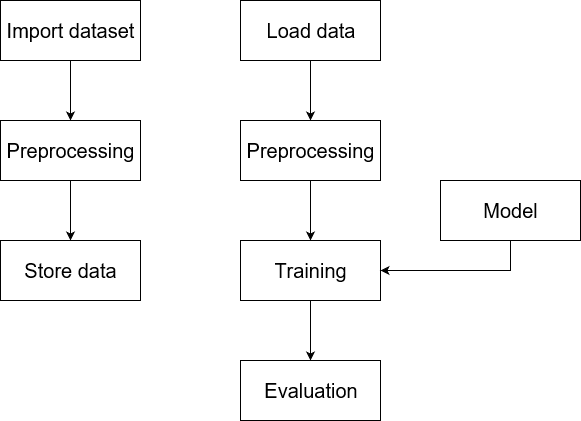
\includegraphics[scale=.4]{figure/block_diag}
	\caption{Framework Pipeline}
	\label{fig:pipeline}
\end{figure}

\section{Signals and Features}
\label{sec:model}

The \textbf{OPPORTUNITY} dataset, succinctly introduced in section \ref{sec:related_work}, has been collected from four subjects accomplishing different Activities of Daily Life (ADLs). As highlighted before, both the subjects and the environment they moved in were meticulously monitored.
The process of acquisition consisted in 5 consecutive runs (named ADL1 to ADL5) that followed a predetermined script, plus a sixth run consisting of 20 repetitions of each of the distinct discrete activity present in the script. Then each vector of samples corresponding to a single time-step is labelled; in the following we'll refer to Task A when we consider an high-level modes of locomotion (\textit{Standing, Walking, Sitting, Lying}) while we'll refer to Task B2 for more specific arm gestures, 17 in total. To these tasks we need of course to add the \textit{Null Class} that we mentioned earlier in this paper: specifically, this label represents the state where the participant does nothing (or something that is not classified among the listed classes). 

The wireless sensors worn by the subjects (IMU - Inertial Measurement Unit) provided acceleration among the three-axes, rate of turn, magnetic field and orientation information; in addition, 12 accelerometers were placed on the subjects' parts of the body sensible to movements (arms, back, hips and feet). All these sensors for a total of 145 distinct acquired channels. \MD{Aggiungere immagine ometti con sensori?}

For the purposes of our work, however, we based the analysis only on on-body sensor signals using just a subset of the available sensors: in this way, we ended up with a total of 113 channels. Another important point is that in the preprocessing phase we performed spline interpolation (which uses a cubic polynomial) in channels that manifested missing data (equivalent to a NaN vale); however, this type of interpolation ends up meaningless if more than the 30\% of data is missing. For this reason we had to discard all the three columns corresponding to one of the physical devices: finally, this led us to work with 110 channels. Since we noticed that the head and tail of the measurement sessions correspond to a transient where most of the sensors are turned-off, we decided to discard them. In this way we ensure that the interpolation phase provides consistent results; the subsequent step consists in normalizing each column with respect to mean and variance. After that, in order to instruct the framework on one subject, we stack sessions from ADL1 to 3 and Drill as a first step to create our training set; then, we assemble also ADL4 and ADL5 to build the test set. 

To conclude the preprocessing phase, finally we decided to follow the same procedure as in several works we cited earlier: we apply in fact the \textit{sliding window} technique on the datasets, obtaining a tensor of windows constituted of \MD{...} samples (\MD{...} ms), using a stride of length \MD{...}. In our case, we decided to assign to each window the most frequent label: this doesn't constitute a problem per se, even when changing the size of the sliding window, as long as it is kept short enough for being representative of a movement.

We found in fact that the choice of window size and stride is fundamental in order to obtain good results: we observed that a window too short can't represent a single gesture with fair precision and, on the contrary, if the window is too large we could include two distinct movements (or modes of locomotion), leading to misplaced classes. The choice of the size of the displacement separating two consecutive windows can guarantee a good trade-off between windows diversity and dataset population.

\section{Learning Framework}
\label{sec:learning_framework}


One of the main problems in Human Activity Recognition is handling \text{inactivity}.

Thinking of a real recognition system, 
In this paper we compare two different learning strategies, mimicking a real system. In the first \ref{sub:oneshot}, \text{One Shot Classification}, the model is trained to learn a representation of the involved classes together with the null class

\subsection{One Shot Classification}
\label{sub:oneshot}

\subsection{Two Steps Classification}
\label{sub:twosteps}
